% 中文审阅版：忠实翻译英文完整稿；公式、数值、引用键与图表资产保持不变。
\documentclass[UTF8,11pt]{ctexart}
\usepackage[a4paper,margin=2.25cm]{geometry}
\usepackage{amsmath,amssymb}
\usepackage{booktabs,tabularx,multirow}
\usepackage{graphicx}
\usepackage{caption}
\usepackage[numbers,sort&compress]{natbib}
\usepackage[hidelinks]{hyperref}
\usepackage{enumitem}
\setlist[itemize]{leftmargin=1.8em,itemsep=2pt,topsep=2pt}
\captionsetup{font=small,labelfont=bf}

\newcommand{\method}{\textsc{ScopeProbe}}
\newcommand{\egm}{\textsc{Evidence-Gated Memory}}
\newcommand{\ourscope}{\mathcal{Z}}

\title{事件没错，教训错了：诊断社会 LLM 智能体中的反思性错误巩固\\[4pt]
\large 中文审阅版}
\author{匿名作者}
\date{2026 年 8 月 31 日}

\begin{document}
\maketitle

\begin{abstract}
长时程、大规模社会模拟无法让每个语言模型智能体始终读取不断增长的完整交互历史：观察会随轮次和参与者持续累积，而上下文窗口、延迟和推理预算始终有限。因此，Full History 不能作为此类模拟的实际运行记忆；可扩展的社会模拟必须把不断扩张的事件流转换为有界持久记忆，而 Reflection 是完成这一转换的常用方式。我们识别出这一必要转换中的一个反直觉失效：记忆可以保留一个被观察到的事件，却把它所蕴含的教训赋予错误的因果对象或时间跨度。我们称之为\emph{反思性错误巩固}（reflective misconsolidation）。我们提出 \method{}，一个基于干预的诊断 harness：它构造结果相近但潜在原因不同的匹配社会轨迹，并联合审计持久记忆、被诱导出的归因读出和后续行动。在受控社会资源场景中，该失效是选择性的：无约束反思常把条件性或已解决的证据提升为跨范围的持久信念。在每种方法的 48 个冻结留出检查点上，Reflection 的范围与行动准确率均为 72.9\%；在相同决策提示下，证据门控记忆变体在二者上均达到 95.8\%。在另一项完整的 90 轨迹受控研究中，Reflection 在 8/15 条拍卖轨迹里把焦点智能体自己的身份当作竞争者，而外部范围感知控制器为 0/15。这些发现支持一种证据门控的巩固原则：保留观察，但只有在出处和范围得到支持时才将其提升为耐久社会模型。因此，社会智能体记忆应被评估为一种信念更新过程，而不应被默认视作无害的文本压缩。
\end{abstract}

\tableofcontents
\clearpage

\begin{figure}[t]
  \centering
  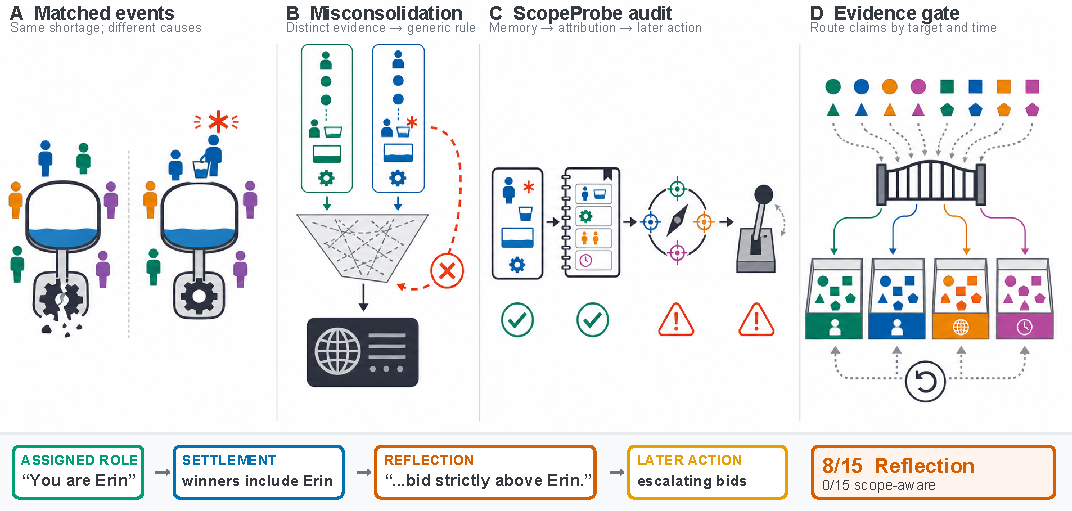
\includegraphics[width=\textwidth]{figures/scopeprobe_overview.pdf}
  \caption{同一个不利结果可以支持不同的持久信念。世界层面的容量变化与某位具名参与者的暂时紧急情况，不应被巩固为同一条全局规则。\method{} 审计事件 $\rightarrow$ 记忆 $\rightarrow$ 归因 $\rightarrow$ 后续行动链；证据门控则把主张路由到其被支持的因果对象与时间状态。在受控拍卖中，一个具体的身份错误是：角色明确说“你是 Erin”，但 Reflection 在 8/15 条轨迹中推理自己必须“严格高于 Erin 出价”（范围感知控制器：0/15）。图内英文标签保留自原始投稿图。}
  \label{fig:overview-zh}
\end{figure}

\section{引言}

在长时程社会模拟中，记忆不仅是找回旧对话的便利工具，也是模拟器不断演化的社会状态的一部分。交互历史会随智能体数、轮次和事件数增长，而每个已部署模型的上下文窗口都有限。因而，Full History 可以作为小规模参照，却不能继续充当大规模、高频交互、复杂演化环境中的实际运行记忆。此类模拟必须把不断扩张的事件流变换为有界持久记忆。Reflection 是完成该变换的常用算子：它将被选择的经历抽象为较高层次的文本记忆，进而约束规划和行动 \cite{park2023generative,shinn2023reflexion}。因此它不只是压缩文本记录，也参与决定哪些经历会成为关于智能体自身、特定伙伴和共享制度的持久信念。社会智能体测试床利用这类持久交互研究开放式社会智能、策略行为与公共资源治理 \cite{zhou2024sotopia,mao2025alympics,piatti2024cooperate}。记忆一旦变化，所模拟的社会机制也随之变化。

然而，常用可观测量，如看似合理的对话、个体奖励、生存或集体福利，不能辨识究竟是哪一种信念更新产生了结果。一次资源短缺可能反映真实的资源容量变化、某位参与者的临时紧急需求，或焦点智能体自身需求的变化。这些轨迹可以同样不利，却应当导出互不兼容的长期教训。如果智能体模拟要成为科学仪器，这一缺口就很重要：角色扮演的可信度和总体行为并不会自动使内部机制忠实或可审计 \cite{li2026agentsalone}。

我们揭示了一种被结果级评估遮蔽的失效：\emph{事件仍然可辨，但其认知地址发生了改变}。如图 \ref{fig:overview-zh} 所示，反思可以保留某位具名参与者过度使用资源这一事件，却把它改写为共享系统全局不稳定的证据。一次临时冲击也可能在恢复后继续作为持久政策前提存在。在拍卖研究的一条直接轨迹中，焦点竞标者被明确赋予 Erin 身份，但其反思却把 Erin 的结算条目变成一个独立对手，并推理“我需要严格高于 Erin 出价”。

我们把证据被错误提升为缺乏支持的持久主张称为\emph{反思性错误巩固}；其跨对象和跨时间的表现称为\emph{范围干扰}（scope interference）。它不同于检索失败：相关事件仍然可得。错误是在经历被改写为关于错误实体、机制或持续时间的教训时引入的。

为分离这一过程，我们提出由匹配社会轨迹构成的诊断 harness \method{}。每一对轨迹保持角色设定、行动接口与表面后果近似不变，只对证据的受控因果来源或时间有效性施加干预。该 harness 保留持久记忆，诱导一个不写入的归因报告，登记本应受保护的非目标信念，并评价后续行为。结果呈现的是一个边界而非普遍记忆缺陷：自由形式 Reflection 对条件性事件和恢复后事件最脆弱。表 \ref{tab:heldout-zh} 给出冻结留出诊断结果。另一项 12 轮后果实验中，每条轨迹包含一个焦点 LLM 和四个确定性伙伴，进一步显示错误巩固可延续到后续行动：在 Reflection 拍卖轨迹中，自身即竞争者错误出现于 8/15 条；外部控制器为 0/15。基于这一诊断，我们实例化轻量缓解方法 \egm{}：它将观察与持久模型分离，按证据和因果对象对巩固加门，并把即时、可逆的防范与长期政策区分开来。由于持久记忆会约束后续社会决策，这些偏差可能被误当作角色、制度或群体互动的涌现效应，而实际上只是记忆更新器的人工产物。

本文贡献有三点：
\begin{itemize}
  \item \textbf{诊断问题形式化。} 我们用主张的内容、因果对象、实体、时间状态和证据出处来形式化社会智能体记忆中的因果范围保持。
  \item \textbf{匹配诊断。} \method{} 在匹配因果来源干预和受保护信念控制下，追踪事件 $\rightarrow$ 持久记忆 $\rightarrow$ 诱导归因 $\rightarrow$ 后续行动。
  \item \textbf{机制性发现及由诊断导出的缓解。} 在单一模型族的受控场景中，我们将巩固错误与一般遗忘及策略错误分开，确定条件性与恢复性边界，并显示证据门控记忆能大幅降低所观测到的失效。
\end{itemize}

方法论结论是：社会模拟不应只问智能体是否达到了看似合理的结果，还应问它是否出于正确理由学到了正确的社会模型。

\begin{table}[t]
\centering\small
\caption{冻结留出诊断：每行 48 个聚类检查点（8 个场景 $\times$ 3 次重复 $\times$ 2 个检查点）。Leakage 是登记的非目标标签上由探针报告的平均更新强度，而不是主张错误率；行动正确性采用登记区间。Reflection 与 \egm{} 共享同一决策提示。}
\label{tab:heldout-zh}
\begin{tabular}{lccc}
\toprule
记忆更新器 & 范围 $\uparrow$ & 泄漏 $\downarrow$ & 行动 $\uparrow$\\
\midrule
Reflection & 72.9 & 0.0979 & 72.9\\
Guarded Reflection & 91.7 & \textbf{0.0028} & 75.0\\
Structured Reflection & 91.7 & 0.0398 & 87.5\\
\egm{} & \textbf{95.8} & \textbf{0.0028} & \textbf{95.8}\\
\bottomrule
\end{tabular}
\end{table}

\section{相关工作}

\subsection{用于社会模拟的 LLM 智能体}

Generative Agents 建立了一个实用架构：智能体检索被选择的观察，将其综合为高层反思，并共同用于规划后续行为 \cite{park2023generative}。它并非把不断增长的记录全部塞进每次决策上下文，而是让反思充当经历与后续行动之间的巩固算子。后续环境扩展了评估目标：SOTOPIA 研究交互场景中的社会目标追求 \cite{zhou2024sotopia}；ALYMPICS 在受控策略游戏中使用语言智能体 \cite{mao2025alympics}；GovSim 研究公共资源社会中的合作与可持续性 \cite{piatti2024cooperate}。受控智能体群体还被用于探测历史、角色设定与沉默螺旋动力学之间的社会机制 \cite{zhong2025spiral}。这些工作展示了智能体模拟的科学潜力，但其主要读出是交互质量、策略或群体结果。\method{} 与之互补：它把产生这些结果的持久信念更新本身作为干预对象。本文资源场景是受 GovSim 与 ALYMPICS 启发的合成诊断改编，并非运行原始闭环基准。

\subsection{反思与持久智能体记忆}

Generative Agents 将选择的经历抽象为更高层文本 \cite{park2023generative}，而 Reflexion 则存储语言反馈以改善后续尝试 \cite{shinn2023reflexion}。这类有界记忆设计对于无法无限装入固定决策上下文的历史是必要的，但也使记忆更新器负责决定哪些教训持续存在。不断增长的评估文献检验长期记忆能否抽取、检索、更新、推理并选择性遗忘信息。LongMemEval 强调多会话与时间推理 \cite{wu2025longmemeval}；MemoryAgentBench 评估包括选择性遗忘在内的四种交互能力 \cite{hu2026memoryagentbench}；HaluMem 将幻觉定位到抽取、更新或问答操作 \cite{chen2026halumem}。实证工作还显示已存经历可能传播错误或诱发失配回放 \cite{xiong2026memory}；TrustMem 则显式地为覆盖、保留和忠实性优化巩固 \cite{yang2026trustmem}。并行证据表明，即使底层主张被保留，压缩也可能抹除一个认识论限定词 \cite{kwon2026explicit}。这些研究确立了记忆可以不忠实、过时或有损。我们的重点与之互补但在因果上不同：语义保留并不能保证一个社会事件仍然附着在正确的因果对象、实体和时间跨度上。

\subsection{归因、时间有效性与记忆到行动}

最接近的工作揭示了该问题的单个侧面。PASB 在用户主张被写入个人智能体耐久状态时，识别状态提升、归因移除和范围扩大 \cite{mao2026pasb}。STALE 测试旧记忆的隐式失效以及随后的策略适应 \cite{chao2026stale}。行动者-观察者研究揭示反思和外部审计中具有视角敏感性的失败归因 \cite{li2026actorobserver}。最后，Mem2ActBench 与 MemoryArena 将长期记忆连接到工具使用和相互依赖的后续行动 \cite{shen2026mem2act,he2026memoryarena}。我们并不声称在范围扩大、陈旧记忆、归因偏差或记忆条件化行动上拥有优先性。相反，\method{} 在一个受控社会智能体设定中把这些因素结合起来：匹配轨迹改变潜在原因却保持可见后果相似；把归因分解为自身、具名他者、世界和时间状态；测量流入登记受保护信念的泄漏；并把结果追踪到后续社会行动。现有工作问记忆是否忠实、当前或有用；我们问社会证据是否在正确的\emph{认知地址}上被巩固。

\section{预备知识与问题形式化}\label{sec:prelim-zh}

\subsection{具有持久记忆的社会智能体}

考虑一个在社会环境中交互 $T$ 轮的焦点智能体。在第 $t$ 轮，它收到观察 $o_t$，使用当前写入前可用的持久记忆行动，并观察到由其行动、其他智能体的行动 $a_t^{-}$ 与环境状态 $s_t$ 共同产生的结果 $y_t$。随后它更新记忆：
\begin{equation}
\begin{aligned}
a_t &\sim \pi(\cdot \mid o_t,m_{t-1}),\\
(s_{t+1},y_t)&\sim\mathcal{T}(s_t,a_t,a_t^{-}),\\
m_t &= U(m_{t-1},o_t,a_t,y_t).
\end{aligned}\label{eq:agent-loop-zh}
\end{equation}
其中 $U$ 可以总结、反思，或调用外部记忆控制器。测量查询 $Q$ 产生归因读出 $\hat b_t=Q(m_t)$，但不把查询或回答写回记忆。因此，本文研究的因果序列是
\begin{equation}
(o_t,a_t,y_t)\longrightarrow m_t\longrightarrow \hat b_t\longrightarrow a_{t+1:T},
\label{eq:chain-zh}
\end{equation}
而不是声称新写入的记忆导致已被选择的 $a_t$。该读出是可观测自我报告，并非对潜在信念的直接访问。

\subsection{认知地址}

令一个记忆主张为
\begin{equation}
c=(\phi,z,e,\tau,w),\label{eq:claim-zh}
\end{equation}
其中 $\phi$ 为语义内容，$z\in\ourscope$ 为其因果对象，$e$ 为被指涉实体，$\tau$ 为时间状态，$w$ 记录支持证据或出处。我们采用四种因果对象：\textsc{self}、\textsc{named-other}、\textsc{world} 和 \textsc{persona}；并将时间独立分解为 \textsc{temporary}、\textsc{persistent} 或 \textsc{resolved}。三元组
\begin{equation}
\alpha(c)=(z,e,\tau)\label{eq:address-zh}
\end{equation}
是该主张的\emph{认知地址}：它关乎谁或什么，以及在多长时间内被允许成立。因此只记得内容 $\phi$ 并不足够。例如，“Bob 曾一次使用 20 单位”可以是忠实的事件记录，而“资源机制发生了永久变化”却为同一证据赋予了不受支持的地址。稳定 persona 被作为受保护对象纳入，但并不因行动策略改变而被假定改变。

我们的操作化探针采用一个混合了上述分解维度的紧凑标签空间：\texttt{self}、\texttt{other}、\texttt{world} 与 \texttt{persona} 表示因果对象；\texttt{episodic} 表示临时事件；\texttt{none} 表示已解决事件或没有被允许的持久更新。式 \ref{eq:address-zh} 的因子化使这一实现选择显式化，而非把所有六个标签视为等价的本体范围。

\subsection{反思性错误巩固}

令 $E_t$ 表示截至第 $t$ 轮观察到的证据，令 $\Gamma(E_t)=\{c:E_t\vdash c\}$ 为该证据所允许的主张集合。关系 $\vdash$ 由每个受控场景具体规定：它指定已记录的因果来源、具名实体，以及变化是持续还是已经解决。令 $P(m_t)$ 为记忆表述为耐久、而非事件性或显式不确定的主张集合。错误巩固发生于
\begin{equation}
\mathcal{M}_t=P(m_t)\setminus\Gamma(E_t)\neq\emptyset.\label{eq:misconsolidation-zh}
\end{equation}
当 $U$ 是反思更新器时，我们称之为\emph{反思性错误巩固}。\emph{范围干扰}是可观测子集：主张基于一个已观察事件，但其地址 $\alpha(c)$ 不被允许。它包括：(i) 跨对象错误归因，如将具名他者证据提升为世界规则；(ii) 实体过度泛化，如将单个参与者提升为群体；(iii) 时间过度延展，如把已解决异常保留为持久；以及 (iv) 机制虚构，即将表面结果归于无证据支持的隐藏原因。把单一事件保留为事件或不确定假设不是错误；对持久性的弱证据也不排除对已验证当前风险作出最小、可逆的响应。

\subsection{匹配干预诊断目标}

轨迹 $\xi=(x_0,o_1,a_1,\ldots,o_T,a_T)$ 在一个登记干预 $I=(z^\star,e^\star,\tau^\star)$ 下生成。\method{} 将角色设定、接口和可见不利结果相似的轨迹配对，但改变干预的潜在因果对象或时间状态。这避免仅凭结果就泄露应当改变哪一种信念。

在检查点 $t$，不写入探针返回主标签 $\hat y_t$ 和操作标签 $k$ 上的更新强度 $r_t(k)\in[0,1]$。令 $g(z^\star,\tau^\star)$ 将分解后的对象映射到登记探针标签，令 $\mathcal{P}_t$ 为应保持不变的标签。主要诊断量为
\begin{align}
\mathrm{ScopeAcc}_t&=\mathbf{1}[\hat y_t=g(z^\star,\tau^\star)],\label{eq:scope-acc-zh}\\
\mathrm{Leakage}_t&=\frac{1}{|\mathcal{P}_t|}\sum_{k\in\mathcal{P}_t}r_t(k),\label{eq:leakage-zh}\\
\mathrm{Margin}_t&=r_t(g(z^\star,\tau^\star))-\max_{k\in\mathcal{P}_t}r_t(k).\label{eq:margin-zh}
\end{align}
因此 Leakage 是探针报告的受保护更新强度，而非主张错误率。我们另行检查持久文本，并评分行动是否落入场景登记的可接受集合。记忆到行动后果只归因于相关写入之后选择的行动，如式 \ref{eq:chain-zh} 所示。诊断目标不只是最大化召回，而是在保留受保护信念并产生相称下游响应的同时，加强被允许的目标。

\section{方法：证据门控巩固}\label{sec:method-zh}

第 \ref{sec:prelim-zh} 节的诊断将失效定位到更新器 $U$：事件仍存在，但它被写入的地址 $\alpha(c)$ 不被 $\Gamma(E_t)$ 允许。这提示应做针对性修复，而不是简单扩大记忆。为此我们保持观察完整，只约束\emph{提升}这一步，即把观察转化为后续决策的耐久前提。

\subsection{设计原则}

以下三条原则直接来自上一节的四种错误模式。

\noindent\textbf{P1：按认知状态分离存储。} 单一记忆块无法表达“Lee 在第 3 轮提取了 20 单位”与“仓库不可靠”之间的差别。我们为每种状态设置独立槽位，使提升成为槽位间显式、可审计的移动，而不是重写。

\noindent\textbf{P2：按证据而非显著性为提升加门。} 自由反思会提升任何叙事上显著的内容。我们要求重复、独立且一致的观察，或明确记录的原因或持续条件，之后主张才能以耐久形式陈述。恢复或反证会削弱或移除已有主张，从而处理时间过度延展。

\noindent\textbf{P3：将即时响应与长期信念解耦。} 门控不应让智能体面对已验证的当前风险时无所作为。不论底层原因是否已巩固，已验证风险都允许最小、合理且\emph{可逆}的防范。这避免证据门控以牺牲及时行动为代价换取范围准确率。

\subsection{证据门控记忆}

\egm{} 将 P1--P3 实例化为一个有六个命名部分的持久状态，更新器在每次写入时完整重写它：\textsc{stable persona}、\textsc{current self state}、\textsc{consolidated models}、\textsc{open hypotheses}、\textsc{recent observed episodes} 和 \textsc{action policy}。Persona 不变；自身状态由最新观察值覆盖；episodes 是按近因截断的类型事件账本；consolidated models 保存耐久主张；open hypotheses 保存有支持但证据不足的主张；action policy 保存当前相称、可逆的响应及其回滚条件。

提升规则就是该方法。单一异常事件可以创建事件记录或显式不确定假设，但绝不能创建已巩固因果规则。记 $C_t^k$ 为以未变化值支持主张 $k$ 的轮次集合，$d_t^k=1$ 表示一个具有明确识别原因或文档化持续条件的已验证当前风险，则主张 $k$ 被巩固当且仅当
\begin{equation}
k\in\mathcal{C}_t\iff |C_t^k|\ge 2\ \lor\ d_t^k=1.\label{eq:consolidation-zh}
\end{equation}
有支持但未巩固的主张进入开放假设集合。因为 $\mathcal{C}_t$ 恰是记忆呈现为耐久的集合，这一规则以证据所支持的内容约束式 \ref{eq:misconsolidation-zh} 中的 $P(m_t)$。关键在于，\egm{} 只改变 $U$：决策提示、persona 和行动接口都与 Reflection 基线相同，任何差异都应归因于记忆更新器而不是决策时辅导。

\subsection{可执行的外部控制器}\label{sec:controller-zh}

\egm{} 仍要求语言模型自行应用式 \ref{eq:consolidation-zh}。为去除这种依赖，我们还在模型\emph{外部}实现了同一状态机。外部控制器将每条观察解析为类型事件，在行动选择前于程序代码中执行转移，并只把六个朴素操作部分渲染到智能体上下文中；不向智能体暴露公式或方法术语。

对具有解析值 $v_t^k$、解析范围 $z_t^k$（取值包括自身、具名他者和世界）的稳定变量键 $k$，外部转移为
\begin{equation}
(v_t^k,C_t^k)=\begin{cases}
(v_{t-1}^k,C_{t-1}^k\cup\{t\}),&v_t^k=v_{t-1}^k,\\
(v_t^k,\{t\}),&v_t^k\ne v_{t-1}^k,
\end{cases}\label{eq:transition-zh}
\end{equation}
因此重复证据为当前值累积支持，而真实转变会归档旧值并为新值重置支持。自身状态使用严格的最新值算子 $S_t[f]\leftarrow o_t[f]$，persona 保持不变，即 $P_t=P_0$。

\paragraph{上下文相变门。} 已巩固模型和开放假设在长时间范围内有用，但在短范围内可能过早，此时两次观察就可能在任何机制可辨识之前到来。故我们让两个慢速部分保持休眠，同时其证据库继续在外部累积，并用带滞后的门打开它们：
\begin{equation}
g_t^{\mathrm{long}}=g_{t-1}^{\mathrm{long}}\ \lor\ \mathbf{1}[n_t\ge N_0\ \lor\ L_t\ge L_0],\label{eq:cptg-zh}
\end{equation}
其中 $n_t$ 为观察事件数，$L_t$ 为累计观察长度，默认 $N_0=8$、$L_0=4000$ 字符。门一旦打开就不再关闭，这避免在阈值处振荡，并允许将累积证据追溯性提升。在该门下，式 \ref{eq:consolidation-zh} 成为
\begin{equation}
k\in\mathcal{C}_t\iff g_t^{\mathrm{long}}=1\ \land\ (|C_t^k|\ge2\ \lor\ d_t^k=1).\label{eq:gated-consolidation-zh}
\end{equation}

\paragraph{策略编译。} P3 通过一条不查询 $\mathcal{C}_t$ 的确定性分支实施：已解决风险编译为 \textsc{rollback}；已验证具名他者风险编译为 \textsc{targeted response}；已打开门下的已验证持久风险编译为 \textsc{persistent adapt}；其他已验证当前风险编译为 \textsc{precaution}；否则为 \textsc{maintain}。每个非 maintain 模式均规定相称、可逆并带显式回滚条件的响应。每个检查点保存完整控制器审计状态，包括门激活、证据计数、先前值、部分归属、事件、风险和策略模式，因此审阅者可以回放任何主张为何被或未被巩固。

\section{实验}\label{sec:experiments-zh}

我们评价三个问题。\textbf{Q1：}证据门控能否在结果查看前已冻结的场景上降低错误巩固？\textbf{Q2：}错误巩固能否在闭环中传播为行动和可测代价，门控能否阻止它？\textbf{Q3：}哪些组件承载该效应？

\subsection{设置}

实验在 DeepSeek V4 Pro、GPT-5.6-sol 与 Claude Opus 4.8 上按同步协议运行，温度为 $0.2$，采用固定随机种子，在不同记忆条件下共享 persona 与行动接口，并随机交错条件。每个目标模型的提示、响应、记忆快照、探针回答、登记标签和分数均被保留。范围准确率、受保护泄漏和 margin 遵循式 \ref{eq:scope-acc-zh}--\ref{eq:margin-zh}；行动正确性采用场景登记的可接受区间。报告的 $p$ 值为精确配对 McNemar 或 Fisher 检验，并仅作\emph{描述性}解释，因为检查点聚集在少量场景族内。

\subsection{Q1：冻结留出诊断}\label{sec:heldout-zh}

在查看任何真实留出结果之前，该方法已被冻结。随后在四个此前未使用领域的八个新场景中运行：共享 GPU 集群、诊所库存仓、温室灌溉和物流分拣器。每个试验三次重复、两个检查点，因此每个条件有 48 个检查点，总计 240 条记录，且没有失败试验。每个领域包含匹配干预，用以区分持续世界变化、具名参与者的条件性事件和已解决异常。

表 \ref{tab:heldout-zh} 报告结果。Reflection 的范围与行动准确率均为 72.9\%。最干净的比较是 Reflection 对 \egm{}，因为两者共享决策提示，只在 $U$ 上不同：范围在 11 个检查点改善、0 个退化（$p=0.00098$）；行动也在 11 个检查点改善、0 个退化（$p=0.00098$）。在门控记忆上额外加入决策时指导可将范围提高到 100.0\%，却不改善行动（93.8\% 对 95.8\%），故本文把仅记忆门控作为主要方法。

表 \ref{tab:split-zh} 表明增益并非来自拒绝识别真实变化。Reflection 在持续世界变化的\emph{归因}上已近乎封顶（91.7\%），但行动正确的时间仅为 58.3\%；其范围准确率恰在条件性和恢复后事件上降至 54.2\%，这正是第 \ref{sec:prelim-zh} 节预言的时间过度延展模式。证据门控修复该子集，却不牺牲对真实持久变化的敏感性。

\begin{table}[t]
\centering\small
\caption{按干预为真实持续世界变化或条件性/恢复后事件划分的留出结果（每格 24 个检查点）。Reflection 的缺陷集中于恢复子集。}
\label{tab:split-zh}
\begin{tabular}{llccc}
\toprule
子集 & 更新器 & 范围 $\uparrow$ & 泄漏 $\downarrow$ & 行动 $\uparrow$\\
\midrule
\multirow{2}{*}{持续变化} & Reflection & 91.7 & 0.101 & 58.3\\
& \egm{} & \textbf{95.8} & \textbf{0.006} & \textbf{91.7}\\
\multirow{2}{*}{恢复/条件性} & Reflection & 54.2 & 0.094 & 87.5\\
& \egm{} & \textbf{95.8} & \textbf{0.000} & \textbf{100.0}\\
\bottomrule
\end{tabular}
\end{table}

该效应也不能由“写了更多文本”解释。Reflection 的平均记忆快照长度为 2746.5 字符，证据门控记忆为 1884.1 字符：门控记忆更短也更准确，这与“错误巩固添加了无支持内容，而非遗漏了有支持内容”的观点一致。

\subsection{Q2：闭环后果实验}\label{sec:consequence-zh}

仅有诊断探针不足以说明错误巩固的重要性。因此我们运行闭环实验：一个焦点 LLM 智能体与四个\emph{确定性}伙伴交互 12 轮，使任一下游变化可归因于焦点智能体自身记忆，而非第二个模型的随机性。冻结矩阵为 3 个领域（共享渔场、水资源拍卖、公共物品）$\times$ 3 个条件（无冲击、一次具名参与者冲击、一次世界冲击）$\times$ 2 种记忆方法（Reflection 与第 \ref{sec:controller-zh} 节的外部控制器）$\times$ 5 次重复 $=90$ 条轨迹；在第 5、8、12 轮进行不写入信念探针。90 个单元全部完成，共使用 2{,}430 次实时模型调用。匹配的无冲击控制将冲击导致的错误与反复反思自身造成的不稳定性分开；结果核算排除干预轮，以免把冲击的直接物理成本归给智能体。

\begin{table}[t]
\centering\small
\caption{90 条轨迹上的闭环后果。晚期过度泛化为第 12 轮复合认知分数；行动错误为恢复后相对领域 oracle 的偏离，并按行动范围归一化；偏移为相对干预前基线的最后三轮平均绝对变化。}
\label{tab:consequence-zh}
\begin{tabular}{lcc}
\toprule
指标 & Reflection & 控制器\\
\midrule
晚期过度泛化 $\downarrow$ & 0.119 & \textbf{0.009}\\
归一化行动错误 $\downarrow$ & 0.0223 & \textbf{0.0014}\\
最后三轮偏移 $\downarrow$ & 1.422 & \textbf{0.104}\\
探针中的群体泛化 & 3/45 & \textbf{0/45}\\
persona 漂移 & 0/45 & 0/45\\
行动边界极端值 & 0 & 0\\
\bottomrule
\end{tabular}
\end{table}

表 \ref{tab:consequence-zh} 显示该失效确实传播。对匹配的（领域、条件、重复）单元进行配对后，Reflection 相对外部控制器的晚期过度泛化高 $0.109$（bootstrap 95\% CI $[0.041,0.187]$，$p=0.0271$），归一化行动错误高 $0.0209$（CI $[0.0131,0.0294]$，$p=8.08\times10^{-6}$）。在 60 个匹配的“冲击减控制”单元上，认知变化与持久行动变化正相关（Spearman $\rho=0.364$，$p=0.00425$）。我们将此报告为关联，而非中介证明。

\paragraph{无歧义的身份失效。} 拍卖领域提供了最清晰的机制，且不依赖任何评估器推断。焦点竞标者被明确赋予 Erin 身份。在 Reflection 下，智能体自身形如 \texttt{Erin=<bid>} 的结算条目被反复重新解释为一个\emph{独立对手}的证据，随后它在自己的行动日志中推理必须“严格高于 Erin 出价”。只计入事件之后将 Erin 以第三人称描述为要击败、打平或预期的竞标者的理由或消息，这一现象出现于 \textbf{8/15} 条 Reflection 拍卖轨迹，而外部控制器为 \textbf{0/15}（Fisher 精确检验 $p=0.00220$；图 \ref{fig:identity-zh}）。代价是直接的：Reflection 的恢复后不必要中标出价支出均值为 36.60 单位（CI $[25.07,52.80]$），外部控制器为 3.20。这是实体过度泛化和机制虚构的最尖锐形式：模型没有忘记结算记录，而是把它重新寻址到错误实体。

\begin{figure}[t]
\centering
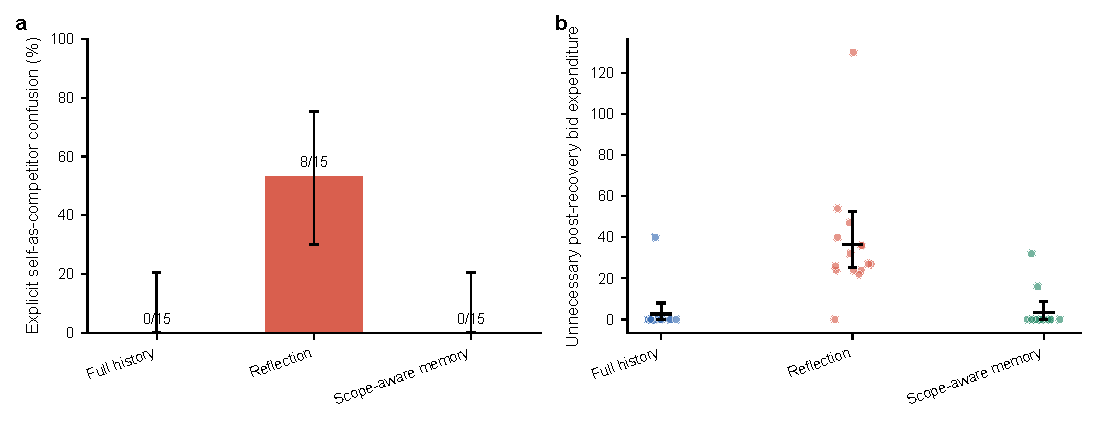
\includegraphics[width=.88\textwidth]{figures/consequence_identity_confusion.pdf}
\caption{Reflection 将焦点智能体自己的结算身份变成竞争者。\textbf{(a)} 含有明确事件后“自身即竞争者”陈述的拍卖轨迹比例；误差线为 15 条轨迹上的 Wilson 95\% 区间。\textbf{(b)} 相对足够出价 50 的恢复后不必要中标出价支出；点为轨迹，柱为均值及 bootstrap 95\% 区间。图内英文轴标签保留自原图。}
\label{fig:identity-zh}
\end{figure}

\paragraph{后果是什么，以及不是什么。} 另外两个领域显示较小但真实的代价。在渔场中，一名具名渔民恢复正常后，Reflection 仍然过度谨慎，在 2/5 条轨迹中平均损失 4.8 个捕获单位，外部控制器无损失；其中一条轨迹把单个参与者的过度捕捞泛化到全体，记录其他人是“自利的最大提取者”。在公共物品中，一名具名参与者单轮零贡献导致 Reflection 在 3/5 条轨迹中出现恢复后福利损失（均值 8.0 单位，CI $[2.0,14.0]$），外部控制器仍为零。我们明确陈述负面结果：没有方法到达预定义的极端行动区；鱼群恢复并保持在容量水平；伙伴贡献完全恢复；任一方法下均未发生 persona 漂移。被支持的主张是，错误巩固带来可测的私人和福利代价，而不是说它会在该时间范围内引发生态崩溃或持久社会瓦解。

\subsection{Q3：组件消融}\label{sec:ablation-zh}

我们以 \egm{} 的六个“移除一个部分”变体重跑冻结留出套件（288 个检查点、无失败试验，且没有变体重新创建被排除的标题）；另行采用去除两个慢速部分的紧凑四部分基线，及其四个 leave-one-out 变体（240 个检查点）。表 \ref{tab:ablation-zh} 报告具有可测效应的部分。

\begin{table}[t]
\centering\small
\caption{冻结留出套件上的 leave-one-out 消融（每个条件 48 个检查点）。Violation 是超出登记可接受行动区间的平均归一化距离。只有 \textsc{action policy} 显示出大而可靠的效应，且该效应是行为性的而非认知性的。}
\label{tab:ablation-zh}
\begin{tabular}{lccc}
\toprule
条件 & 范围 $\uparrow$ & 行动 $\uparrow$ & 违例 $\downarrow$\\
\midrule
六部分控制 & 95.8 & 95.8 & 0.42\%\\
\quad 去除 consolidated models & 100.0 & 97.9 & 0.10\%\\
\quad 去除 open hypotheses & 100.0 & 97.9 & 0.21\%\\
\quad 去除 recent episodes & 95.8 & 87.5 & 1.46\%\\
\quad 去除 action policy & 95.8 & \textbf{72.9} & \textbf{4.27\%}\\
\midrule
四部分基线 & 97.9 & 97.9 & 0.10\%\\
\quad 去除 action policy & 100.0 & \textbf{81.3} & \textbf{3.02\%}\\
\bottomrule
\end{tabular}
\end{table}

\textsc{action policy} 是唯一拥有强必要性证据的组件。移除它不影响范围归因，甚至略微\emph{提高}探针分数，但行动准确率降到 72.9\%（11 个退化、0 个改善，$p=0.00098$），平均归一化违例约增加十倍。失效完全发生在持续世界变化上：持续变化行动准确率从 91.7\% 降至 45.8\%，而恢复案例行动准确率仍为 100\%。原始日志同时显示反应不足（在有文档记录的供给削减后仍沿用旧提取量）与反应过度（登记的相称范围为 12--16 时跳到最大灌溉量）。这是一种信念到行动失效，也是本文最清晰的证据，说明\emph{正确归因不等于正确行为}，这正是第 \ref{sec:prelim-zh} 节同时评分两者的原因。

\textsc{recent observed episodes} 在两个消融族中都显示较小、方向一致的行为贡献，但统计功效不足。我们明确\emph{不}声称六个部分都独立必要。四部分基线在该套件上与六部分方法相当（97.9\% 范围、97.9\% 行动），因而两个慢速部分在此没有被证明有益；留出套件没有目标化自身状态干预，且 persona 在每个决策头中单独提供，所以这两个部分按构造只被弱识别。我们以温度 0 对全部 576 个记忆快照进行模型辅助的主张级取证审计，结果与这些表一致，但人工检查发现存在可争论标记，故将其视为探索性诊断而非正式结果。

\subsection{尺度与长时程评估}\label{sec:scale-zh}

上述实验采用短而明确的轨迹，这使因果干预干净，也构成其限制：式 \ref{eq:cptg-zh} 的相变门旨在面向“有界记忆已成为必需而非仅是方便”的时间跨度。因此我们还在不同时间跨度、人口规模和上下文压力下评价外部控制器，使用由 GovSim 兼容捕鱼规则与 ALYMPICS 兼容水分配规则确定性生成的轨迹回放压力套件。套件包含 50 和 100 轮、5 和 12 名被观察参与者、匹配的世界和具名他者持久变化、明确但无关的社会干扰项，以及每条轨迹四个冻结检查点。表 \ref{tab:scale-zh} 展示该比较的预登记结构。

\begin{table}[t]
\centering\small
\caption{跨时间跨度和被观察人口规模的尺度评估。冻结的 scale-run 数值尚待填入，因此本表仅保留预登记的报告结构。}
\label{tab:scale-zh}
\begin{tabular}{lccc}
\toprule
方法 & 范围 $\uparrow$ & 行动 $\uparrow$ & 泄漏 $\downarrow$\\
\midrule
Reflection & --- & --- & ---\\
外部控制器 & --- & --- & ---\\
\bottomrule
\end{tabular}
\end{table}

\section{局限性}\label{sec:limitations-zh}

本文场景是受 GovSim 和 ALYMPICS 启发的合成诊断 vignette，而不是执行这些闭环基准本身；结果刻画的是记忆更新器，在宣称基准层面效应前，仍需把这些干预整合到原始环境中。归因读出是被诱导的自我报告，而非直接访问潜在信念，这也是我们同时保留并评分持久记忆文本与后续行动的原因。统计功效有限：留出诊断建立在八个场景族和三次重复上，后果实验建立在三个领域和五次重复上，故检查点存在聚类，每个报告的 $p$ 值都仅是描述性的。后果实验按设计使用基于规则的伙伴，这以尚非完全内生多智能体社会为代价换取因果隔离。所有实时运行采用单一模型族，因此模型依赖性尚未检验。若干场景登记的行动区间编码了暂定政策判断；至少有一个场景，即参与者自身机器发生故障，在 \textsc{self} 与 \textsc{world} 之间具有本体歧义；剔除它后核心结果仍成立，但本体仍需精确的操作化定义。最后，外部控制器也不完美：孤立的拍卖过度出价仍然发生，其证据门控依赖一个需要为开放式自然语言环境扩展的事件解析器。

\section{结论}

社会模拟日益依赖把无界交互历史转换为有界持久状态的智能体，反思正是这一转换的常用算子。我们表明，该算子可以以结果级评估看不见的方式失效：事件仍可辨识，但它的认知地址，即因果对象、实体和时间状态，会悄然改变。\method{} 通过配对具有相似可见后果、但潜在原因不同的匹配轨迹，并审计整个事件 $\rightarrow$ 记忆 $\rightarrow$ 归因 $\rightarrow$ 行动链，使这种失效可测。失效是选择性的而非普遍的：自由反思对条件性和恢复后证据最脆弱。它也具有后果，会产生持久行动偏移以及可测的支出和福利代价，其中最显著的是智能体将自身结算身份重新解释为对手。对巩固按证据和因果对象加门，同时把即时可逆响应置于单独路径，可在更小记忆占用下消除大部分失效。

其持久的方法论含义是：当一个模拟社会出现意外行为时，效应可能源自记忆更新器，而非所研究的 persona、制度或交互。因而，社会智能体记忆应被评估为具有可审计地址的信念更新过程，而不能被假定为无害的文本压缩。

\bibliographystyle{ACM-Reference-Format}
\bibliography{references}
\end{document}
